\section{Background}
\label{sec:back}

\if 0
The display technology used by mobile devices started from monochrome display
to liquid crystal display (LCD) to the present technology of organic
light-emitting diode (OLED).
In the LCD the brightness of the screen is regulated by a backlight. With the
advent by OLED the brightness was depended on the pixel with are lighted.
\fi

\paragraph{Frame rendering.}
% Figure~\ref{fig:arch} illustrates the frame rendering process in a
% typical modern smartphone.  After the GPU renders a new frame, \eg
% every 16.7ms at 60 FPS, the bitmap of the frame content is stored in
% the frame buffer and sent to the hardware composer. The hardware
% composer before sending the final bitmap to
% the hardware display.  Each unit of the bitmap describes the color of
% a pixel in the standard RGB (sRGB) color space, ($R, G,
% B)$, which specifies the intensities of the red, green, and blue base
% colors.  Modern displays come with 24-bit (8, 8, 8) RGB color setting,
% \ie each intensity ranges between 0 and 255.
Figure~\ref{fig:arch} illustrates the frame rendering process in a
typical modern smartphone~\cite{arch_graphicspipeline}.
After the GPU renders all the layers for the next frame
(for status bar, navigation bar, and app UI),
\eg every 16.7ms at 60 FPS, 
the bitmap of the frame content is stored in separate buffer queues.
%
Each unit of the bitmap describes the color of
a pixel in the standard RGB (sRGB) color space, ($R, G,
B)$, which specifies the intensities of the red, green, and blue base
colors.  Modern displays come with 24-bit (8, 8, 8) RGB color setting,
\ie each intensity ranges between 0 and 255.
%
SurfaceFlinger provides HardwareComposer HAL with a list of layers and
instructs it to compose the final frame sent to the display.
HardwareComposer HAL may perform additional color transformation to
generate the final frame.

If the Android screenrecord command is issued, SurfaceFlinger composes
the multiple layers from buffer queues into a frame
buffer~\cite{arch_surfaceflinger} sent to an additional virtual
display for screen recording. Note that such recorded frame buffers would not
include color transformation happening in HardwareComposer below.

%  The Hardware Composer HAL (HWC) composite buffers in the most
%  efficiently specific to device display hardware.


%  and may not be the true representation
%  of the device display, as it is handled by SufaceFlinger.  Hence, the
%  color mode, color correction and brightness changes are not captured
%  by virtual display.

\begin{figure}[tp]
  \centering
        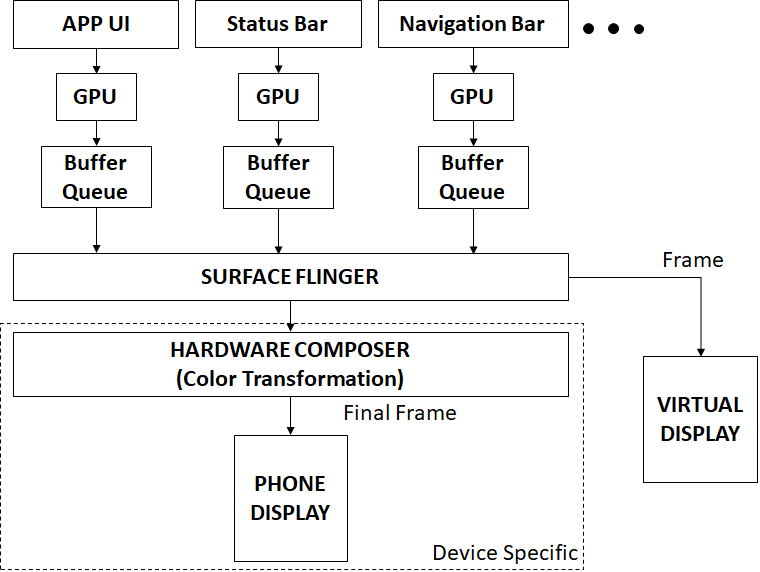
\includegraphics[width=0.45\textwidth]{./figure/1400_architecture.png}
        \vspace{-0.1in}
	\caption{Frame rendering in modern smartphones.}
        \vspace{-0.2in}
        \label{fig:arch}
\end{figure}

\forjnl{Organic light-emitting diode (OLED), also known as an organic EL
  (organic electroluminescent) diode~\cite{oled:2003,oled:2004}, is a light-emitting
diode (LED) in which the emissive electroluminescent layer is a film
of organic compound that emits light in response to an electric
current.}
%
\if 0
offer several
significant advantages: (1) OLED enables a greater contrast ratio and
wider viewing angle compared to LCD, because OLED pixels emit light
directly. In particular, OLED provides a deeper black level, since a
black OLED display emits no light, while
 LCD cannot show true black, since it filters the light emitted from a backlight.
 (2) OLED
 \fi
% Further, OLED pixel colors appear correct and unshifted, even as the viewing angle approaches 90° from the normal.
\forjnl{ The ability of OLED pixels to emit light omits the need for external
 backlight needed in LCD and provides much better power efficiency than LCD.
}


\paragraph{OLED display.}
Each pixel of an OLED display consists of three subpixels,
corresponding to red, green, and blue colors, which
can differ significantly in their luminance
efficacies~\cite{oled:2003,oled:2004}.  This is the reason why the color of a pixel determines
its power consumption and thus different display content (\eg different
app UI design) can result in very different OLED display power draw.
\forjnl{This is in stark contrast with LCD displays where the (external) back
lighting dominates the whole display power.
}

In addition to the panel of addressable pixels, the total OLED display
power consumption is affected by the control circuitry
that generates the control and data signals for the panel based on
display contents. Different circuitry implementation can potentially
result in different power draw.
%   There are two main families of OLED, based on small molecules
%   and polymers, respectively.
%   Adding mobile ions to an OLED creates a
%   light-emitting electrochemical cell (LEC) which has a slightly
%   different mode of operation.
\if 0
{An OLED display can be driven with a passive-matrix (PMOLED) or
active-matrix (AMOLED) control scheme.  For example, ??? and ?????
phones use PMOLED and PIXEL 2 and Moto Z3 phones use AMOLED. In the PMOLED
scheme, each row (and line) in the display is controlled serially, one
by one~\cite{pmoled:amoled}. In contrast, AMOLED control uses a
thin-film transistor backplane to directly access and switch each
individual pixel on or off, allowing for higher resolution and larger
display sizes.
}
\fi

\if 0
\paragraph{Applications of OLED power models.}
An accurate OLED power model can be used to isolate the power draw of
the OLED display of a smartphone, which has many useful applications,
such as energy profiling of mobile
apps~\cite{appscope,zhang2010accurate,shye2009into,pathak:eurosys12,mittal:mobicom12}
and component-wise energy accounting of online tools such as Android
Battery~\cite{???}.
\fi

\if 0
\subsection{Problem Statement}
\label{subsec:problem}

Since the OLED display power draw depends on the pixel values of the
displayed frame, our goal is to develop an OLED power model that {\em
  given a frame of pixels, can accurately estimate the OLED power draw
  in displaying the frame}.  Such a model needs to satisfy two
requirements:
%\begin{itemize}%[noitemsep,leftmargin=*]
  \begin{itemize}[leftmargin=*]
\item {\em Accurate:} For the model to be useful, it needs to be accurate, ideally within a few percent
of the ground truth;
\item {\em Efficient:} Modern phone displays come with millions of pixels.
The runtime for applying the OLED model to a given
frame should be fast, ideally within a few milliseconds, \ie a fraction of
the time each new frame is generated (16.7ms for 60 FPS),
so that it can be used online with low overhead, \eg in Abdroid Battery,
or used in offline processing where the OLED energy of a recorded screen video
should be processed in a fraction of the video duration.
\end{itemize}
  \fi
  

\paragraph{OLED power modeling.}
Since an OLED display consists of $N$ pixels that emit lights
independently of each other, the total power draw of an OLED display
equals the sum of the power draw $P_i$ by individual pixels
(\eg~\cite{dong2009current,kim2013runtime}):
\begin{equation}
	P_{OLED} = C + \sum_{i=1}^{n}{P_i}
	\label{eq:linear_equation0}
\end{equation}
where constant $C$ is used to account for the 
% base power drew by
power draw by
the non-pixel component of the OLED display,
denoted as {\em dark screen power},
and individual pixel power draw $P_i$ depends on
the pixel color value.

To use an OLED power model, the screen needs to be recorded and
fed into the model.  Ideally, we want to record the final frame 
sent to the display.  However, Android only provides interfaces that record
the frame buffer (via virtual display)  which will miss possible
color transformation in the hardware composer.  We discuss the implications
on OLED power modeling in \S\ref{subsec:brightness} and
\S\ref{subsec:colortransform}.


\if 0
Eqn.~\ref{eq:linear_equation0} rests on two assumptions:

\noindent
{\bf Assumption 1:} The non-pixel component of the OLED display power $C$ is independent
of the pixel values;

\noindent
{\bf Assumption 2:} The power draw of the pixel component of the OLED display $P_i$
are independent of each other.
\fi


